\documentclass[11pt,a4paper,oneside]{book}

\usepackage[utf8]{inputenc}
\usepackage[T1]{fontenc}
\usepackage[italian,english]{babel}
\usepackage{graphicx}
\usepackage{hyperref}
\usepackage{amsmath, amsfonts, amssymb}
\usepackage{geometry}
\usepackage{tcolorbox}
\usepackage{booktabs}
\usepackage{tabularx}
\usepackage{array}
\usepackage{float}
\usepackage{listings}
\usepackage{xcolor}
\usepackage{fancyhdr}
\usepackage{titlesec}
\usepackage{microtype}

\geometry{a4paper, top=3cm, bottom=3cm, left=3cm, right=3cm}
\setlength{\headheight}{14.5pt}

% Configurazione header e footer
\pagestyle{fancy}
\fancyhf{}
\fancyhead[L]{\nouppercase{\leftmark}}
\fancyhead[R]{\thepage}

% Configurazione cartella immagini
\graphicspath{{images/}{img/}}

% Configurazione Listings per Codice Java / Akka
\definecolor{codegreen}{rgb}{0,0.6,0}
\definecolor{codegray}{rgb}{0.5,0.5,0.5}
\definecolor{codepurple}{rgb}{0.58,0,0.82}
\definecolor{backcolour}{rgb}{0.97,0.97,0.97}

\lstdefinestyle{mystyle}{
    backgroundcolor=\color{backcolour},   
    commentstyle=\color{codegreen},
    keywordstyle=\color{blue}\bfseries,
    numberstyle=\tiny\color{codegray},
    stringstyle=\color{codepurple},
    basicstyle=\ttfamily\footnotesize,
    breakatwhitespace=false,         
    breaklines=true,                 
    captionpos=b,                    
    keepspaces=true,                 
    numbers=left,                    
    numbersep=5pt,                  
    showspaces=false,                
    showstringspaces=false,
    showtabs=false,                  
    tabsize=2,
    frame=single,
    rulecolor=\color{lightgray}
}
\lstset{style=mystyle}

% Stile link
\hypersetup{
    colorlinks=true,
    linkcolor=black,
    filecolor=magenta,      
    urlcolor=blue,
    citecolor=blue,
    pdftitle={Networked Software for Distributed Systems},
    pdfauthor={Riccardo Nasatti}
}


\begin{document}

% Frontespizio
\begin{titlepage}
    \centering
    \vspace*{2cm}
    {\Large \textbf{Politecnico di Milano}}\\[0.5cm]
    {\large Master of Science in Computer Science and Engineering}\\[2.5cm]

    {\Huge \textbf{Networked Software for\\Distributed Systems}}\\[1cm]
    {\LARGE Comprehensive Course Notes \& Lab Preparation}\\[2.5cm]

    {\large \textbf{Docenti:}}\\
    {\large Prof. Luca Mottola \quad Prof. Alessandro Margara}\\[2cm]

    \vfill
    {\large \textbf{Autore:}}\\
    {\large Riccardo Nasatti}\\[1.5cm]

    {\large Anno Accademico 2026/2027}
    \vspace*{1.5cm}
\end{titlepage}

\tableofcontents
\clearpage

\chapter{The Actor Model and Akka}

\section{Foundations of Concurrent and Distributed Computing}

\subsection{The Concurrency Crisis and the Shared-Memory Paradigm}
Modern computing architectures are fundamentally parallel. As physical constraints—primarily thermal dissipation limits and power density ceilings (the "power wall")—halted the scaling of single-core clock frequencies, hardware manufacturers transitioned to multi-core, many-core, and distributed architectures. Consequently, achieving high-throughput and low-latency software execution necessitates concurrent execution models.

Historically, the predominant abstraction for concurrent programming on shared-memory platforms has been multi-threading coupled with explicit synchronization primitives (such as mutual exclusion locks, semaphores, monitors, and atomic memory operations). Under this model, concurrent threads share a unified address space, accessing and mutating shared variables directly. However, this approach exhibits severe mathematical and engineering pathologies:
\begin{enumerate}
    \item \textbf{Non-Deterministic Interleaving and Race Conditions}: The execution order of concurrent memory access is governed by the underlying operating system thread scheduler and hardware memory models (e.g., store buffers, out-of-order execution, and compiler optimizations). If two threads access a shared memory location concurrently without adequate synchronization, and at least one access is a write, a data race occurs. Detecting, reproducing, and debugging such race conditions is notoriously difficult due to non-deterministic scheduling.
    \item \textbf{Deadlocks, Livelocks, and Lock Contention}: Coordinating access to multiple shared resources requires strict, globally enforced lock acquisition hierarchies to prevent circular wait conditions (the Coffman conditions for deadlock). As system scale grows, maintaining global locking hierarchies becomes intractable. Fine-grained locking introduces high synchronization latency, CPU cache bouncing, and high risk of deadlocks, while coarse-grained locking severely serializes execution, collapsing concurrent throughput.
    \item \textbf{Violations of Object-Oriented Encapsulation}: In standard Object-Oriented Programming (OOP), an object encapsulates state and invariants, exposing methods to manipulate that state. However, in a multi-threaded shared-memory environment, an object's boundary is entirely porous: multiple threads of execution can simultaneously execute the object's methods, mutating private fields without intrinsic boundary isolation. Thus, object-oriented encapsulation fails to protect state invariants under concurrent execution.
    \item \textbf{Lack of Spatial and Network Portability}: Shared-memory synchronization primitives rely inherently on shared physical RAM, atomic hardware instructions (e.g., Compare-And-Swap - CAS), and unified cache-coherence protocols. These abstractions cannot cross network boundaries. Consequently, code written using thread locks cannot be transitioned to a distributed cluster without an architectural rewrite.
\end{enumerate}

\subsection{The Actor Model: A Mathematical Paradigm of Message-Driven Concurrency}
To overcome the intrinsic failures of shared-memory multi-threading, Carl Hewitt, Peter Bishop, and Richard Steiger proposed the \textbf{Actor Model} in 1973, subsequently formalized and extended by Gul Agha (1986). The Actor Model treats the \textbf{Actor} as the universal primitive of concurrent and distributed computation.

Joe Armstrong, the co-inventor of Erlang, encapsulated the core philosophy of actor-oriented programming:
\begin{quote}
\textit{“The world is parallel. If we want to write programs that behave as other objects behave in the real world, then these programs will have a concurrent structure. Use a language that was designed for writing concurrent applications, and development becomes a lot easier. Erlang programs model how we think and interact.”}
\end{quote}
Complementing this, the modern engineering ethos (articulated in the Effective Go paradigm and embraced by actor systems) dictates:
\begin{quote}
\textit{“Do not communicate by sharing memory; instead, share memory by communicating.”}
\end{quote}

In the formal Actor Model, an actor is an autonomous computational entity that encapsulates:
\begin{itemize}
    \item \textbf{Private State}: The internal variables of an actor are strictly confined to its execution context. No other entity in the entire system can inspect, read, or mutate an actor's private state directly.
    \item \textbf{A Mailbox}: A message queue associated with the actor where incoming messages are buffered until processed.
    \item \textbf{A Message Handler (Behavior)}: A function that dictates how the actor reacts to incoming messages.
\end{itemize}

Formally, in response to receiving a message from its mailbox, an actor can execute a finite set of operations strictly restricted to:
\begin{equation}
\mathcal{A}(\text{Message}) \longrightarrow \begin{cases}
1. & \text{Create a finite set of new actors: } \{\mathcal{A}'_1, \mathcal{A}'_2, \dots, \mathcal{A}'_k\}, \\
2. & \text{Send a finite set of messages to known actor addresses: } \{(\text{Target}_i, \text{Msg}_i)\}_{i=1}^m, \\
3. & \text{Designate the replacement behavior/state } \beta_{\text{next}} \text{ for the next message.}
\end{cases}
\end{equation}

\begin{figure}[htbp]
\centering
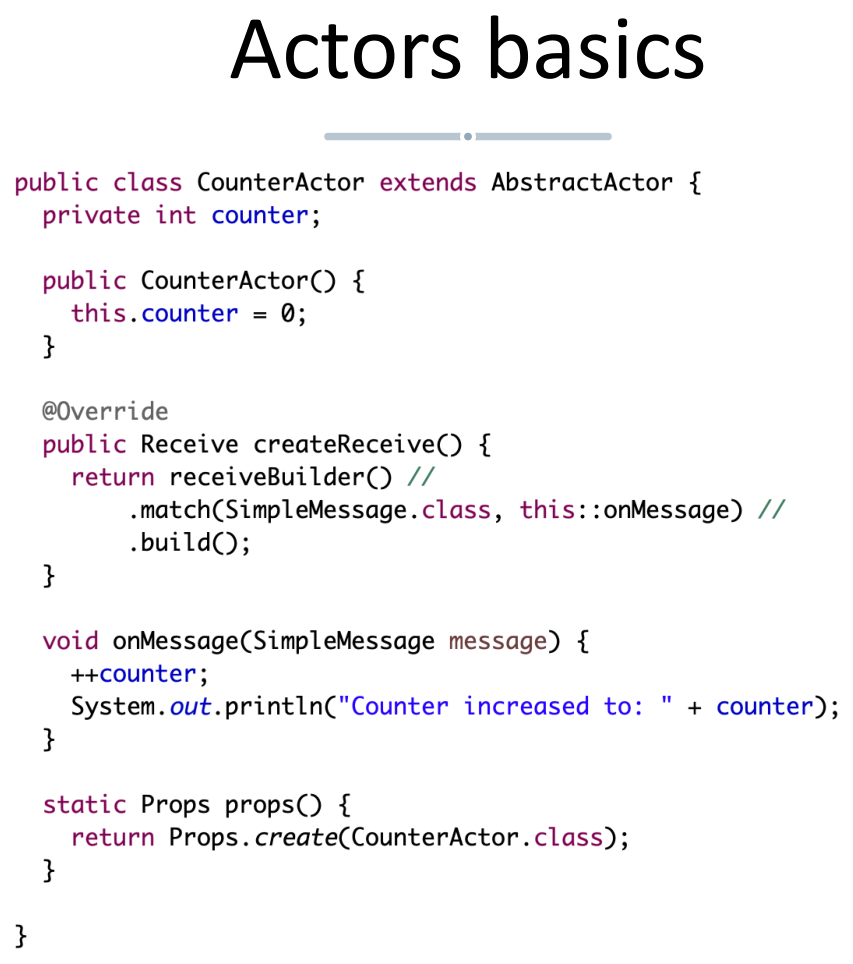
\includegraphics[width=0.65\textwidth]{img/chapter_01/deck1_slide_20.png}
\caption{Architectural structure of an Actor: incoming messages queue into the private mailbox, processed sequentially by the message handler with complete state isolation.}
\label{fig:actor_model_primitive}
\end{figure}

\subsection{Key Invariants and Mathematical Properties of Actors}
The operational semantics of the Actor Model enforce several critical theoretical properties:
\begin{itemize}
    \item \textbf{Thread Confinement and Absence of Shared Mutable State}: Actors never share state variables. Communication occurs exclusively via asynchronous message passing. Because an actor processes exactly one message at a time sequentially from its mailbox, the actor body is entirely free from internal data races. No synchronized blocks, mutexes, or atomic primitives are ever required within an actor's business logic.
    \item \textbf{Atomic Message Processing}: The processing of an individual message is atomic with respect to the actor's state: the actor processes the message from start to finish without interleaving with other messages in that actor. Incoming messages arriving concurrently are queued into the mailbox.
    \item \textbf{Asynchrony}: Message transmission is natively asynchronous (non-blocking). When Actor $A$ sends a message to Actor $B$, Actor $A$ does not block waiting for Actor $B$ to receive or process the message. It resumes its own execution immediately.
    \item \textbf{Stateful and Persistent}: Actors maintain mutable state across sequential message invocations. Furthermore, in persistent implementations (such as Akka Persistence), an actor's state can be snapshotted or reconstructed via event sourcing from durable storage.
    \item \textbf{Spatial and Topological Transparency}: Actors interact using logical addresses (\textbf{Actor References}) rather than physical memory pointers or socket handles. The communication syntax is identical whether the recipient resides on the same CPU core, in the same JVM process, on a different server in the local data center, or across a global wide-area network.
\end{itemize}

\subsection{Industrial Provenance and Adoption}
The actor model is not merely a theoretical construct; it forms the technological backbone of ultra-reliable, high-scale telecommunication and enterprise distributed systems:
\begin{itemize}
    \item \textbf{Erlang / OTP}: Developed at Ericsson by Joe Armstrong to power telecommunication switches requiring "nine nines" ($99.9999999\%$) availability. It powers WhatsApp (enabling billions of concurrent connections with minimal hardware footprints), Apache CouchDB, and RabbitMQ.
    \item \textbf{Microsoft Orleans}: A virtual actor framework powering the global backend cloud infrastructure for multiplayer gaming systems such as \textit{Halo}.
    \item \textbf{Akka (JVM - Java and Scala)}: Created by Jonas Bonér and Lightbend, Akka provides a high-performance actor runtime on the Java Virtual Machine. It is deployed in mission-critical distributed production systems by enterprises including BMW, Volkswagen Group, Siemens, Bosch, and Volvo.
\end{itemize}

---

\section{The Akka Actor Architecture on the JVM}

\subsection{Core Components of the Akka Ecosystem}
Akka translates the formal Actor Model into an enterprise-grade JVM framework. The runtime consists of four foundational abstractions:
\begin{enumerate}
    \item \textbf{ActorSystem}: The heavyweight container and root context for an actor application. It allocates shared resources, including thread pools, dispatchers, configuration parameters, dead-letter mailboxes, and scheduler services. Typically, an application instantiates exactly one \texttt{ActorSystem} per JVM process:
    \begin{lstlisting}[language=Java]
ActorSystem system = ActorSystem.create("NSDS-System");
    \end{lstlisting}
    \item \textbf{Props}: An immutable configuration object that specifies the recipe for creating an actor instance, including the actor's implementation class, constructor parameters, and dispatcher assignment.
    \item \textbf{ActorRef}: An immutable, serializable logical handle (reference) to an actor. Client code and peer actors never interact with the raw Java object instance of an actor; all interaction is strictly mediated through \texttt{ActorRef}. An \texttt{ActorRef} remains valid even if the underlying actor restarts due to a failure.
    \item \textbf{AbstractActor}: The base class in Java used to implement custom actor behavior by defining the message-handling loop in the \texttt{createReceive()} method.
\end{enumerate}

\begin{figure}[htbp]
\centering
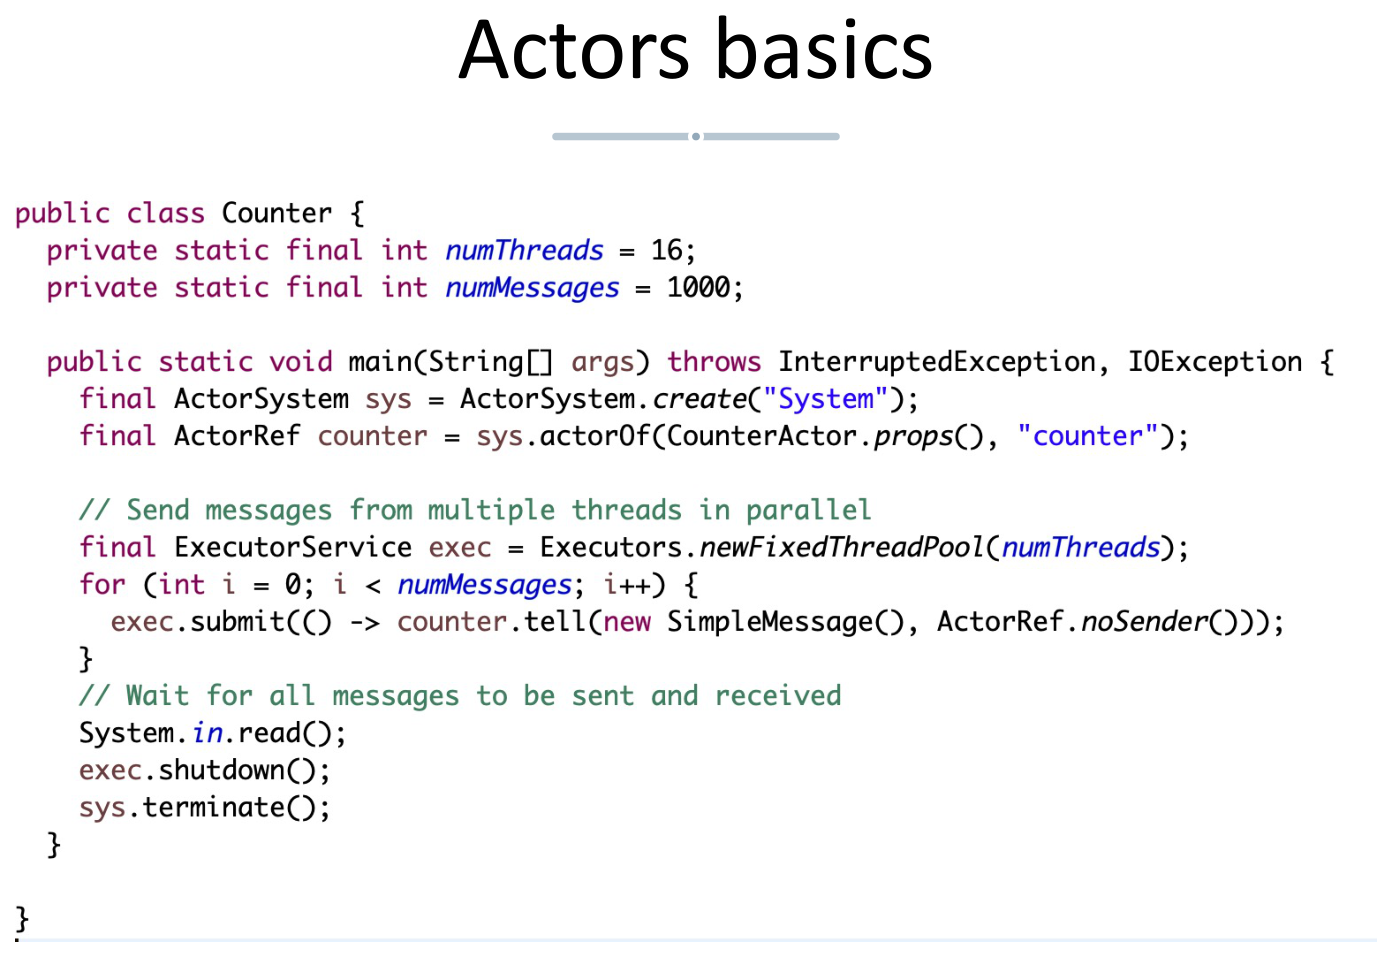
\includegraphics[width=0.75\textwidth]{img/chapter_01/deck1_slide_21.png}
\caption{Decoupling of ActorRef, Mailbox, and Actor Instance: clients interact strictly through ActorRef, shielding the concrete actor instance from direct method invocation.}
\label{fig:actorref_decoupling}
\end{figure}

\subsection{Creating Actors and the Static Props Pattern}
To instantiate an actor, the \texttt{ActorSystem} or an existing actor context must be invoked using the \texttt{actorOf} factory method, passing a \texttt{Props} instance and an optional unique string name.

In Akka with Java, best practice dictates implementing a static factory method \texttt{props()} inside the actor class to ensure type safety and encapsulate constructor arguments:
\begin{lstlisting}[language=Java]
public class CounterActor extends AbstractActor {
    private int counter;

    public CounterActor(int initialValue) {
        this.counter = initialValue;
    }

    // Static Props factory method
    public static Props props(int initialValue) {
        return Props.create(CounterActor.class, () -> new CounterActor(initialValue));
    }

    @Override
    public Receive createReceive() {
        return receiveBuilder()
            .match(IncrementMessage.class, msg -> {
                this.counter += msg.getDelta();
            })
            .build();
    }
}
\end{lstlisting}

Actors are instantiated in client code as:
\begin{lstlisting}[language=Java]
ActorSystem system = ActorSystem.create("ClusterSystem");
ActorRef counterRef = system.actorOf(CounterActor.props(0), "counterActor");
\end{lstlisting}

\subsection{Actor Lifecycle and Lifecycle Hooks}
An actor in Akka progresses through distinct lifecycle phases: \textbf{Starting}, \textbf{Receiving / Executing}, \textbf{Restarting} (upon failure), and \textbf{Stopped}. The framework provides explicit lifecycle callbacks that can be overridden to manage resources, open/close network sockets, or initialize internal state:

\begin{table}[htbp]
\centering
\small
\begin{tabularx}{\textwidth}{l p{4.5cm} X}
\toprule
\textbf{Lifecycle Method} & \textbf{Invocation Trigger} & \textbf{Operational Semantic \& Typical Usage} \\
\midrule
\texttt{preStart()} & Immediately after actor creation, before the first message is processed. & Initialization of private state, establishing external socket/database connections, scheduling recurring timer messages. \\
\midrule
\texttt{preRestart(reason, message)} & Invoked on the failing actor instance right before it is terminated during a restart directive. & Disposes of allocated external resources; by default terminates all child actors and calls \texttt{postStop()}. \\
\midrule
\texttt{postRestart(reason)} & Invoked on the newly instantiated actor instance immediately after restart. & Re-initializes state for the new instance; by default calls \texttt{preStart()}. \\
\midrule
\texttt{postStop()} & Invoked immediately after the actor has been completely stopped and removed from the hierarchy. & Final cleanup, releasing OS handles, notifying remote monitors, flushing buffers to disk. \\
\bottomrule
\end{tabularx}
\caption{Akka Actor Lifecycle Callback Hooks.}
\label{tab:lifecycle_hooks}
\end{table}

\begin{figure}[htbp]
\centering
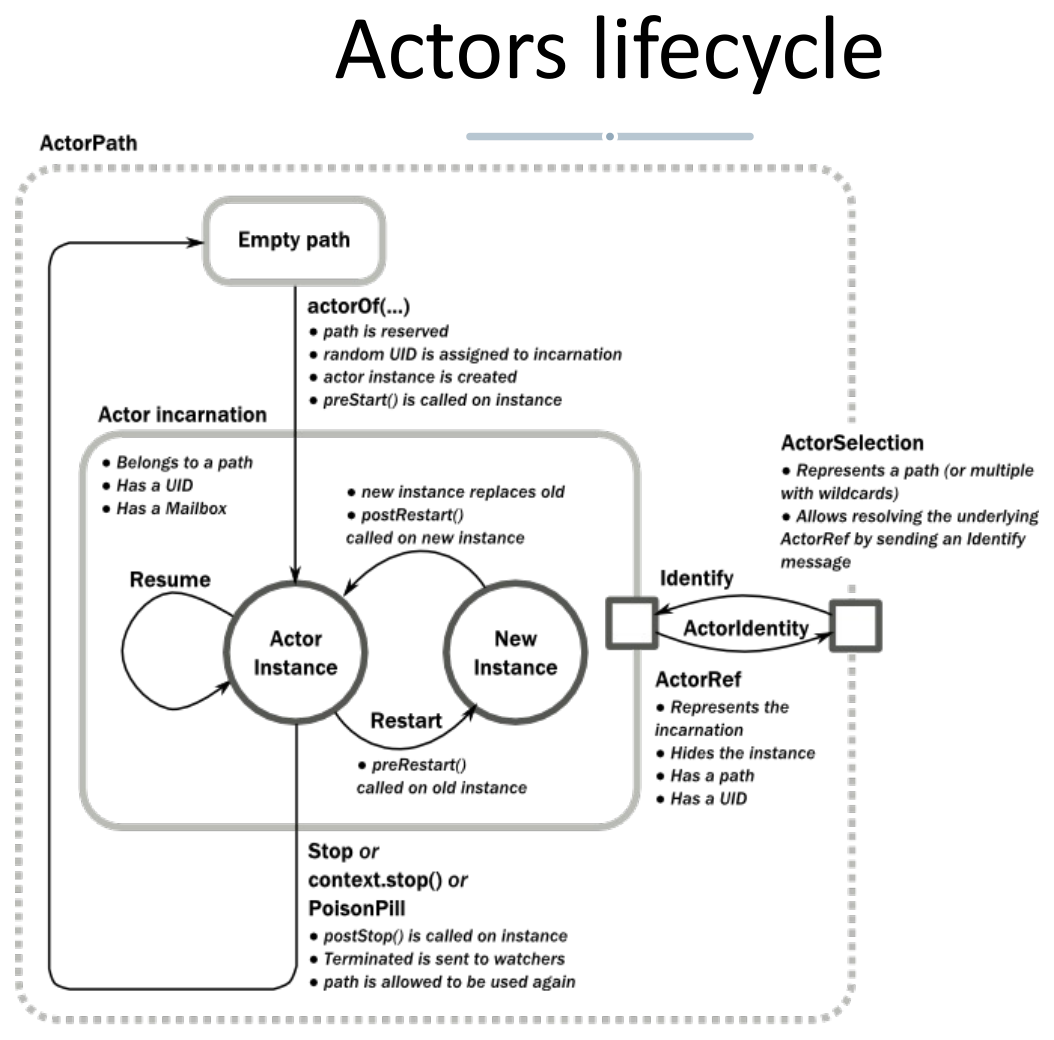
\includegraphics[width=0.7\textwidth]{img/chapter_01/actor_lifecycle.png}
\caption{State machine depicting the complete lifecycle transitions of an Akka actor instance, highlighting restart and termination loops.}
\label{fig:actor_lifecycle}
\end{figure}

\subsection{Mailbox Semantics and the Immutability Requirement}
Each actor is assigned a \textbf{Mailbox} upon creation. The default mailbox implementation is unbounded and enforces \textbf{FIFO (First-In, First-Out)} queuing discipline per sender-receiver pair.

\subsubsection{Ordering Guarantees}
In Akka, message ordering satisfies the following formal guarantees:
\begin{enumerate}
    \item \textbf{Pairwise FIFO Ordering}: If Actor $A$ sends message $M_1$ and subsequently message $M_2$ to Actor $B$, then $M_1$ will always be delivered to Actor $B$'s mailbox and processed before $M_2$, provided direct local dispatch or reliable point-to-point network channels (e.g., TCP) are used:
    \begin{equation}
    \text{Send}_A(M_1 \prec M_2) \implies \text{Receive}_B(M_1 \prec M_2)
    \end{equation}
    \item \textbf{Non-Deterministic Cross-Sender Interleaving}: If Actor $A$ sends message $M_A$ to Actor $C$, and Actor $B$ sends message $M_B$ to Actor $C$, there is no guaranteed relative ordering between $M_A$ and $M_B$. The arrival order depends entirely on network transit latency and thread scheduling non-determinism.
\end{enumerate}

\subsubsection{The Imperative of Immutable Messages}
Because Akka actors executing on the same JVM share a heap memory space, message references passed between actors on the same machine are transmitted as direct memory pointers for maximum performance (avoiding serialization overhead). Consequently:
\begin{quote}
\textbf{All messages exchanged between actors MUST be strictly immutable.}
\end{quote}
If a message object contains mutable fields (e.g., public setters, exposed arrays, or mutable collections), two actors executing on separate dispatcher threads could concurrently read and mutate the message payload, resurrecting the very data races, memory visibility bugs, and cache inconsistencies that the Actor Model mathematically eliminates.

Java does not statically enforce immutability at compile time. Therefore, developers must enforce the following pattern:
\begin{lstlisting}[language=Java]
// Canonical Immutable Message Pattern
public final class TemperatureReadingMsg implements Serializable {
    private final String sensorId;
    private final double temperature;
    private final long timestamp;

    public TemperatureReadingMsg(String sensorId, double temperature, long timestamp) {
        this.sensorId = sensorId;
        this.temperature = temperature;
        this.timestamp = timestamp;
    }

    public String getSensorId() { return sensorId; }
    public double getTemperature() { return temperature; }
    public long getTimestamp() { return timestamp; }
}
\end{lstlisting}

\subsubsection{Unhandled Messages and Dead Letters}
In the \texttt{createReceive()} builder, match clauses are evaluated in the order in which they are declared. If an incoming message matches no clause, Akka triggers the \texttt{unhandled(Object message)} handler. The default implementation publishes the unhandled message to the \texttt{ActorSystem}'s \textbf{Dead Letters Event Stream}. Messages addressed to terminated or non-existent actors are similarly routed to Dead Letters.

---

\section{Communication Patterns, Protocols, and Location Transparency}

\subsection{The Tell Pattern (Asynchronous Fire-and-Forget)}
The primary primitive for message transmission is \texttt{tell()}:
\begin{lstlisting}[language=Java]
targetActorRef.tell(message, senderActorRef);
\end{lstlisting}
The \texttt{tell()} operation is completely asynchronous and non-blocking: it enqueues the message into the target actor's mailbox and immediately returns control to the caller thread.

Key operational semantics:
\begin{itemize}
    \item \textbf{Sender Identification}: When sending from within an actor, passing \texttt{self()} as the second argument enables the receiver to reply using \texttt{sender().tell(replyMsg, self())}.
    \item \textbf{No Sender}: When sending from outside an actor (e.g., from a static \texttt{main} method), passing \texttt{ActorRef.noSender()} indicates that no response is expected:
    \begin{lstlisting}[language=Java]
counterActor.tell(new IncrementMessage(1), ActorRef.noSender());
    \end{lstlisting}
    \item \textbf{Message Forwarding}: An actor can forward a message to a third-party actor while preserving the original sender reference using \texttt{forward()}:
    \begin{lstlisting}[language=Java]
workerActor.forward(message, getContext());
    \end{lstlisting}
\end{itemize}

\subsection{The Ask Pattern (Asynchronous Request-Reply with Futures)}
While \texttt{tell()} represents the pure actor paradigm, software often requires interacting with non-actor boundaries (e.g., handling incoming HTTP requests, orchestrating synchronous integration tests, or querying an actor from the \texttt{main()} thread). For these scenarios, Akka provides the \textbf{Ask Pattern} via \texttt{akka.pattern.Patterns.ask}:

\begin{lstlisting}[language=Java]
import static akka.pattern.Patterns.ask;
import scala.concurrent.Future;
import scala.concurrent.Await;
import scala.concurrent.duration.Duration;
import java.util.concurrent.TimeUnit;

Duration timeout = Duration.create(3, TimeUnit.SECONDS);
Future<Object> future = ask(targetActorRef, new QueryBalanceMsg(accountId), 3000);

// Synchronously blocking the calling thread until completion or timeout
BalanceResponse reply = (BalanceResponse) Await.result(future, timeout);
\end{lstlisting}

\subsubsection{Internal Mechanics and Performance Overhead of Ask}
Under the hood, the Ask Pattern does not alter the recipient actor's execution:
\begin{enumerate}
    \item Akka instantiates an ephemeral, single-use \textbf{Promise Actor} within the \texttt{ActorSystem}.
    \item The message is sent to the target actor with the Promise Actor's reference passed as the implicit \texttt{sender()}.
    \item A timer is registered with the system scheduler for the specified timeout duration.
    \item When the target actor replies via \texttt{sender().tell(response, self())}, the Promise Actor receives the reply, fulfills the underlying Scala/Java \texttt{Future}, and immediately terminates.
    \item If the timeout expires before a reply arrives, the Future fails with an \texttt{AskTimeoutException}.
\end{enumerate}

\begin{table}[htbp]
\centering
\small
\begin{tabularx}{\textwidth}{l X X}
\toprule
\textbf{Dimension} & \textbf{The Tell Pattern (\texttt{tell})} & \textbf{The Ask Pattern (\texttt{ask})} \\
\midrule
\textbf{Execution Model} & Purely asynchronous, non-blocking fire-and-forget. & Asynchronous returning a Future; can be blocked via \texttt{Await.result()}. \\
\midrule
\textbf{Resource Overhead} & Extremely lightweight: enqueues directly into recipient's mailbox. & Medium: allocates a temporary Promise Actor, a timer, and a Future handle. \\
\midrule
\textbf{Failure Handling} & Transparent: network drop or crash handled via supervisor or dead letters. & Explicit: fails with \texttt{AskTimeoutException} if target crashes or drops message. \\
\midrule
\textbf{Best Used For} & Internal actor-to-actor communication, high-throughput pipelines. & Bridging non-actor code to actors (e.g., REST endpoints, \texttt{main} tests). \\
\bottomrule
\end{tabularx}
\caption{Comparative Analysis: Tell Pattern vs. Ask Pattern.}
\label{tab:tell_vs_ask}
\end{table}

\subsection{Delivery Guarantees: Why Best-Effort (At-Most-Once)?}
Distributed systems theory establishes that in the presence of unreliable network channels, guaranteeing exactly-once delivery without coordination overhead is impossible (the Two Generals' Problem).

Akka adopts a strict \textbf{at-most-once (best-effort)} delivery semantic by default:
\begin{itemize}
    \item Messages may be lost if an actor crashes, if a mailbox overflows, or if a network link partitions.
    \item Messages are never duplicated by the transport layer itself.
\end{itemize}

\textbf{Architectural Justification ("Less is More")}:
As emphasized by Professor Mottola, providing at-least-once or guaranteed delivery at the transport layer imposes severe costs: sequence numbering, acknowledgment packets, retransmission buffers, state persistence, and deduplication caches. In distributed environments:
\begin{enumerate}
    \item The underlying Internet Protocol (IP) is natively best-effort.
    \item TCP provides reliable byte-streams over single connections, but cannot mask machine crashes, network partitions, or process restarts.
    \item Many domain operations are naturally idempotent or time-sensitive (e.g., periodic sensor telemetry, where a dropped packet is superseded by the next reading).
    \item Applications requiring stronger guarantees can implement application-level acknowledgments and retries, or integrate durable message queues (such as Apache Kafka).
\end{enumerate}

\subsection{Location Transparency and Akka Remoting}
One of the most powerful architectural capabilities of Akka is \textbf{Location Transparency}. An actor reference (\texttt{ActorRef}) encapsulates identity independently of physical topology. Whether an actor resides on the local JVM or on a remote node across a network, message invocation remains syntactically identical: \texttt{ref.tell(msg, self())}.

\subsubsection{Actor Paths and Hierarchical Addressing}
Every actor is uniquely identified by an \textbf{Actor Path}, structured analogously to a hierarchical filesystem URI:
\begin{equation}
\texttt{akka.<protocol>://<actor-system-name>@<hostname>:<port>/user/<actor-hierarchy-path>}
\end{equation}
For example:
\begin{itemize}
    \item Local path: \texttt{akka://NSDS-System/user/supervisor/worker-1}
    \item Remote TCP path: \texttt{akka.tcp://ClusterNode@192.168.1.100:2552/user/dataProcessor}
\end{itemize}

\subsubsection{Configuring Remote Nodes via HOCON}
Akka uses the Human-Optimized Config Object Notation (HOCON) for configuration (typically in \texttt{application.conf}):
\begin{lstlisting}
akka {
  actor {
    provider = remote
  }
  remote {
    enabled-transports = ["akka.remote.netty.tcp"]
    netty.tcp {
      hostname = "127.0.0.1"
      port = 6123
    }
  }
}
\end{lstlisting}

\subsubsection{Resolving Remote Actors: ActorSelection}
To communicate with a remote actor whose \texttt{ActorRef} is not yet locally available, a client program resolves the remote actor's logical URI using \texttt{actorSelection}:
\begin{lstlisting}[language=Java]
// Client lookup of remote server actor
String remoteAddress = "akka.tcp://ServerSystem@127.0.0.1:6123/user/serverActor";
ActorSelection remoteSelection = getContext().actorSelection(remoteAddress);

// Messages can be sent directly to an ActorSelection
remoteSelection.tell(new QueryMessage("data"), getSelf());
\end{lstlisting}
Once the remote actor replies, the local actor acquires the remote actor's concrete \texttt{ActorRef} via \texttt{sender()}, enabling direct, cached communication without subsequent URI resolutions.

---

\section{Dynamic Behavior Switching and the Stash Mechanism}

\subsection{Finite State Machines via the Become/Unbecome Pattern}
In many concurrent protocols, an actor must fundamentally alter how it reacts to incoming messages depending on its operational state (e.g., transitioning from \textit{Disconnected} to \textit{Connecting}, \textit{Active}, \textit{Busy}, or \textit{Suspended}).

Rather than cluttering message handling logic with complex, error-prone conditional branches (\texttt{if-else} or \texttt{switch} statements inspecting internal status flags), Akka empowers actors to dynamically swap their entire message-handling function at runtime using \texttt{getContext().become()}:

\begin{lstlisting}[language=Java]
public class ProtocolActor extends AbstractActor {

    @Override
    public Receive createReceive() {
        return disconnectedBehavior();
    }

    private Receive disconnectedBehavior() {
        return receiveBuilder()
            .match(ConnectMsg.class, msg -> {
                // Perform connection logic...
                System.out.println("Connecting to " + msg.getHost());
                getContext().become(connectedBehavior());
            })
            .match(DataMsg.class, msg -> {
                System.err.println("Rejected data: Not connected!");
            })
            .build();
    }

    private Receive connectedBehavior() {
        return receiveBuilder()
            .match(DataMsg.class, msg -> {
                System.out.println("Processing data: " + msg.getPayload());
            })
            .match(DisconnectMsg.class, msg -> {
                System.out.println("Disconnecting...");
                getContext().become(disconnectedBehavior());
            })
            .build();
    }
}
\end{lstlisting}

The \texttt{become()} method accepts a second boolean parameter, \texttt{discardOld} (defaulting to \texttt{true}). If set to \texttt{false}, Akka pushes the new behavior onto an internal behavior stack. The actor can subsequently revert to its previous behavior by invoking \texttt{getContext().unbecome()}.

\subsection{The Stash Mechanism: AbstractActorWithStash}
Often, an actor in a particular operational state cannot immediately process certain incoming messages, yet discarding them would violate application protocol requirements. The \textbf{Stash} pattern enables an actor to set aside messages temporarily and replay them later when its state permits.

To utilize stashing, an actor must:
\begin{enumerate}
    \item Inherit from \texttt{AbstractActorWithStash} (or implement the \texttt{Stash} trait).
    \item Invoke \texttt{stash()} on messages that must be deferred. This removes the current message from the active dispatch loop and appends it to a private, secondary stash buffer.
    \item When transitioning to an operational state capable of handling deferred messages, invoke \texttt{unstashAll()}.
\end{enumerate}

\subsubsection{Internal Mailbox Repositioning Semantics}
When \texttt{unstashAll()} is executed, Akka transfers all messages currently in the stash buffer back into the actor's primary mailbox. Crucially:
\begin{quote}
\textbf{Stashed messages are prepended to the front of the primary mailbox in the exact order in which they were stashed.}
\end{quote}
This guarantees that stashed messages are processed immediately upon behavior transition, ahead of newly arriving messages, preserving local causal progression.

\begin{figure}[htbp]
\centering
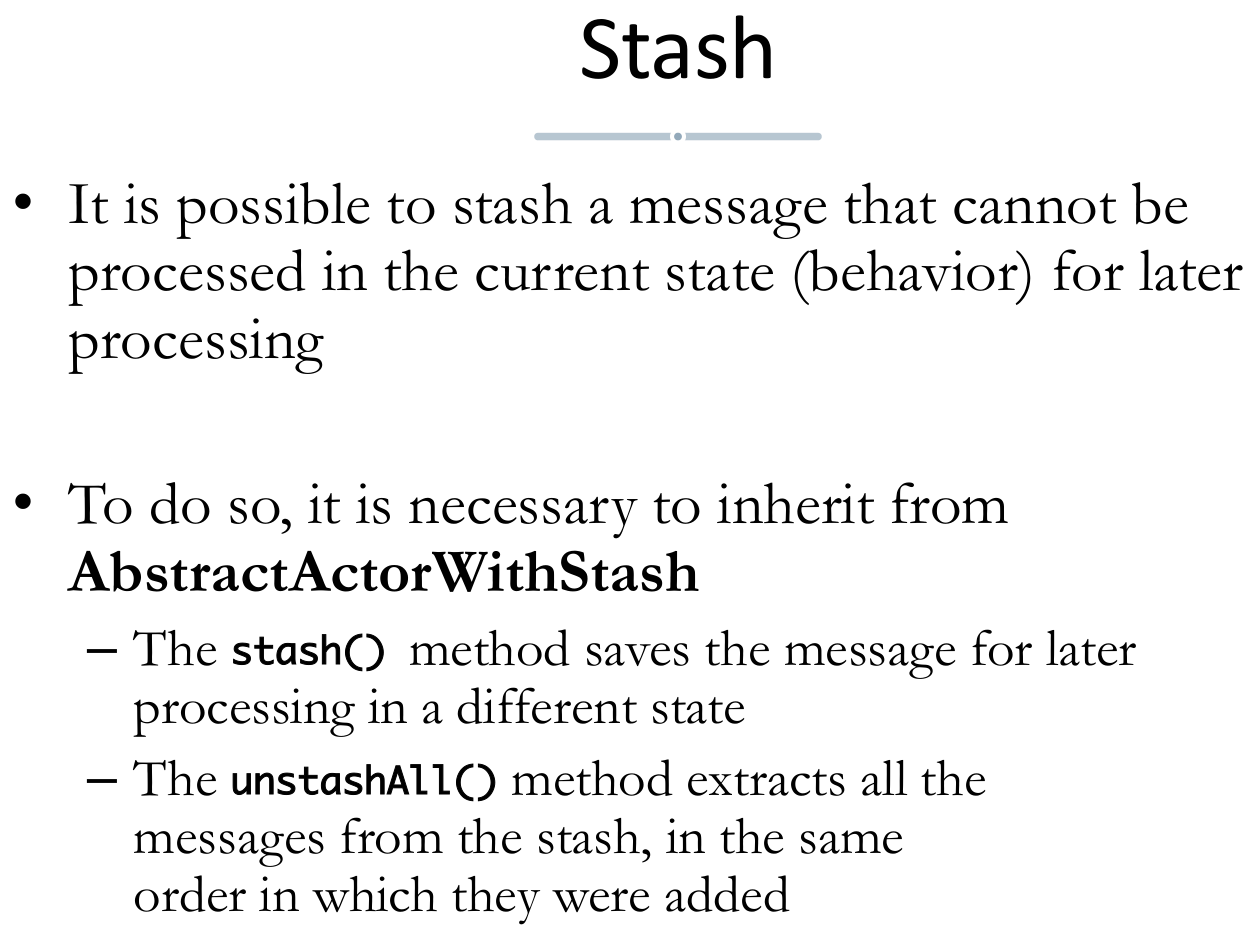
\includegraphics[width=0.75\textwidth]{img/chapter_01/stash_mechanics.png}
\caption{The Stash buffer mechanics: deferred messages are stashed and later prepended to the primary mailbox upon unstashAll().}
\label{fig:stash_mechanics}
\end{figure}

---

\section{Fault Tolerance and the Supervision Hierarchy}

\subsection{The "Let It Crash" Philosophy}
In traditional monolithic programming (e.g., standard Java), error handling is tightly coupled with business logic through defensive \texttt{try-catch} blocks. When an unhandled exception propagates up the call stack, threads crash unpredictably, frequently leaving shared data structures corrupted or locks permanently held.

The Actor Model adopts Joe Armstrong’s radical \textbf{"Let It Crash"} philosophy:
\begin{itemize}
    \item \textbf{Decoupling Error Handling from Business Logic}: Developers do not write defensive code attempting to handle catastrophic failures inside the core message processing loop. If a fatal runtime anomaly occurs (e.g., database connection dropped, corrupted payload, null pointer), the actor simply throws an exception and crashes.
    \item \textbf{Supervision from Outside}: Fault management is completely externalized. When an actor crashes, its parent in the actor hierarchy—its \textbf{Supervisor}—is automatically notified by the Akka runtime and makes an architectural decision on how to recover.
\end{itemize}

\subsection{The Actor Hierarchy}
In Akka, actors do not exist in isolation; they are organized into a strict tree hierarchy. Every actor created via \texttt{getContext().actorOf()} is a child of the actor that created it.

\begin{figure}[htbp]
\centering
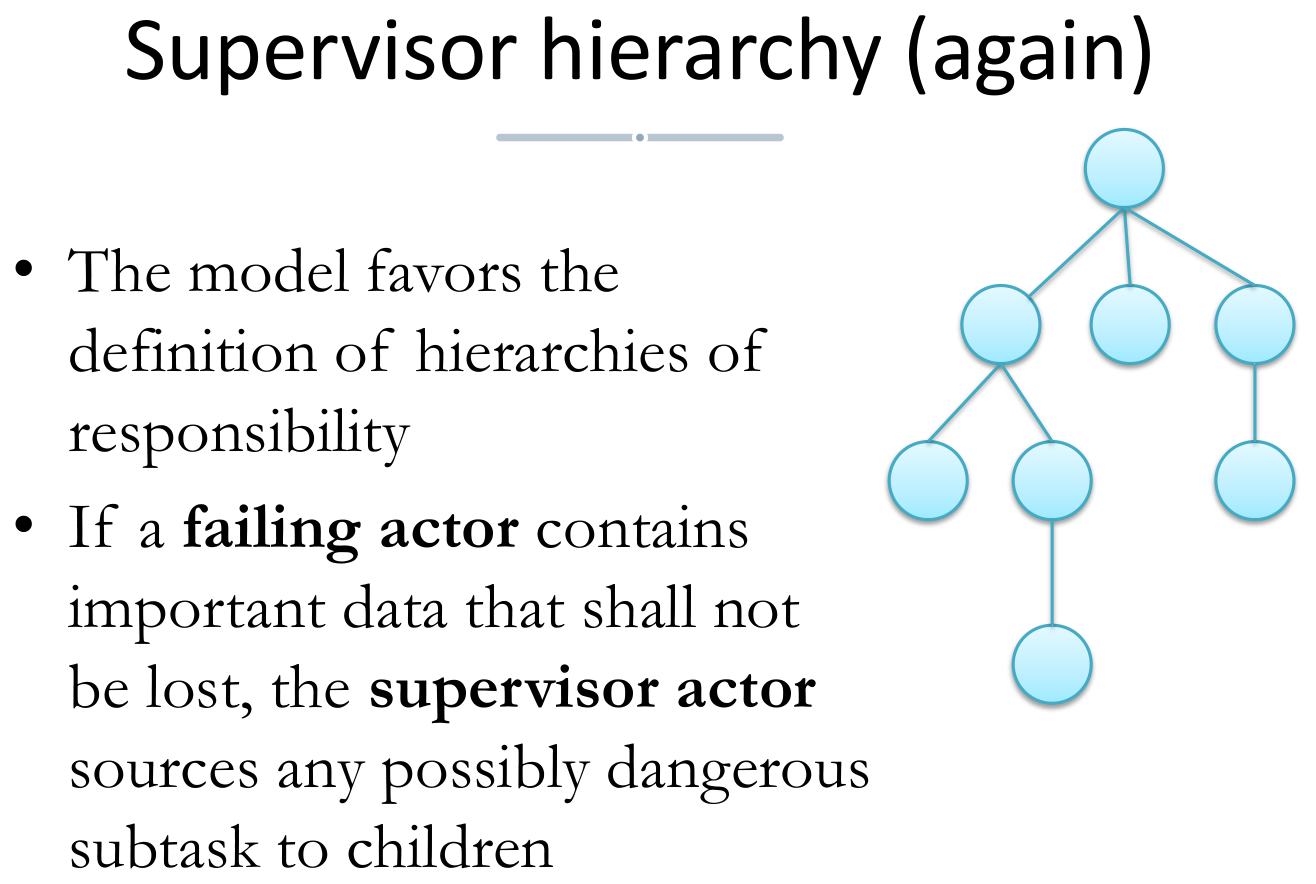
\includegraphics[width=0.75\textwidth]{img/chapter_01/deck3_slide_6.png}
\caption{The Akka Supervision Tree Hierarchy: showing Root Guardian, User Guardian (/user), and nested application supervisor/worker topologies.}
\label{fig:supervision_hierarchy}
\end{figure}

The hierarchy consists of three structural tiers:
\begin{enumerate}
    \item \textbf{Root Guardian (\texttt{/})}: The top of the hierarchy, supervising the internal system guardians.
    \item \textbf{System Guardian (\texttt{/system})}: Manages internal framework services, logging actors, remoting endpoints, and dead letters.
    \item \textbf{User Guardian (\texttt{/user})}: The parent of all top-level application actors created via \texttt{system.actorOf()}. Every user-defined actor has a supervisor.
\end{enumerate}

\subsection{Supervision Strategies and Directives}
A supervisor defines its recovery policy by overriding the \texttt{supervisorStrategy()} method, returning an instance of either \texttt{OneForOneStrategy} or \texttt{AllForOneStrategy}:

\begin{itemize}
    \item \textbf{OneForOneStrategy}: The recovery directive chosen by the supervisor is applied \textbf{only} to the specific child actor that crashed. Peer child actors continue operating without disruption. This is the optimal strategy when children perform independent workloads.
    \item \textbf{AllForOneStrategy}: The recovery directive chosen by the supervisor is applied to \textbf{all} child actors belonging to that supervisor, even if only one child failed. This strategy is mandatory when child actors participate in a tightly coupled, cooperative transaction where the failure of one invalidates the collective state of the group.
\end{itemize}

\subsubsection{The Four Supervisory Directives}
Upon intercepting a child failure, the supervisor executes one of four formal directives:
\begin{enumerate}
    \item \textbf{Resume}: The crashed actor instance is \textbf{not} terminated. It retains its entire private in-memory state and immediately proceeds to process the next message in its mailbox.
    \begin{itemize}
        \item \textit{Use Case}: Minor, transient, or non-state-corrupting anomalies (e.g., a temporary network timeout, a malformed sensor packet that can be discarded without invalidating historical aggregates).
    \end{itemize}
    \item \textbf{Restart} (\textit{Default Policy}): The failing actor instance is destroyed and a brand-new instance of the actor class is instantiated via its original \texttt{Props}.
    \begin{itemize}
        \item \textit{State Semantic}: The actor's private state is completely reset to its initial condition.
        \item \textit{Mailbox Semantic}: The actor's mailbox is \textbf{preserved}. Unprocessed messages remain queued, and the new instance processes them sequentially.
        \item \textit{Lifecycle Hook Invocations}: The old instance executes \texttt{preRestart(reason, message)}; the new instance executes \texttt{postRestart(reason)}.
        \item \textit{Use Case}: State corruption or unrecoverable local exceptions where re-initializing from a clean slate restores operational integrity.
    \end{itemize}
    \item \textbf{Stop}: The failing actor instance is permanently terminated. Its mailbox is drained (unprocessed messages are redirected to Dead Letters), all its child actors are recursively terminated, and its \texttt{ActorRef} becomes defunct.
    \begin{itemize}
        \item \textit{Use Case}: Unrecoverable failures, critical resource exhaustion, or terminal operational errors.
    \end{itemize}
    \item \textbf{Escalate}: The supervisor confesses inability to handle the exception, escalating the failure up the hierarchy to its own parent supervisor. The supervisor itself suspends its own operation and all its children while waiting for its parent's directive.
\end{enumerate}

\subsubsection{Defining a Supervision Strategy in Code}
The following complete Java implementation demonstrates configuring a \texttt{OneForOneStrategy} with retry limits and time windows:

\begin{lstlisting}[language=Java]
import akka.actor.AbstractActor;
import akka.actor.OneForOneStrategy;
import akka.actor.SupervisorStrategy;
import akka.japi.pf.DeciderBuilder;
import java.time.Duration;

public class CustomSupervisorActor extends AbstractActor {

    // Strategy: maximum 10 retries within a 1-minute moving window
    private static final SupervisorStrategy STRATEGY = new OneForOneStrategy(
        10,
        Duration.ofMinutes(1),
        DeciderBuilder
            .match(IllegalArgumentException.class, e -> SupervisorStrategy.resume())
            .match(NullPointerException.class, e -> SupervisorStrategy.restart())
            .match(IllegalStateException.class, e -> SupervisorStrategy.stop())
            .matchAny(e -> SupervisorStrategy.escalate())
            .build()
    );

    @Override
    public SupervisorStrategy supervisorStrategy() {
        return STRATEGY;
    }

    @Override
    public Receive createReceive() {
        return receiveBuilder()
            .match(Props.class, childProps -> {
                // Spawning a supervised child actor
                ActorRef child = getContext().actorOf(childProps);
                sender().tell(child, self());
            })
            .build();
    }
}
\end{lstlisting}

---

\section{Akka Clustering and Distributed Topology}

\subsection{Decentralized Cluster Membership Architecture}
Akka Cluster extends location transparency across a dynamic pool of networked nodes without relying on centralized coordination masters (such as Apache ZooKeeper). It provides:
\begin{itemize}
    \item \textbf{Decentralized Peer-to-Peer Topology}: All nodes are symmetric members; there is no single point of failure (SPOF) or central bottleneck.
    \item \textbf{Gossip Protocol}: Cluster membership state is disseminated asynchronously through periodic, randomized pairwise state gossip.
    \item \textbf{Failure Detection}: Automatic, distributed monitoring of node reachability.
\end{itemize}

\subsection{The Gossip Protocol and Vector Clock Convergence}
Nodes organize into an overlay network. At regular intervals (default: 1 second), each node randomly selects another cluster member and exchanges membership views.
\begin{itemize}
    \item \textbf{Vector Clocks for Causal History}: Each gossip message includes a \textbf{Vector Clock} tracking the partial order of membership state modifications observed across nodes (e.g., nodes joining, leaving, or becoming unreachable).
    \item \textbf{Gossip Convergence}: A node attains cluster state convergence when it can mathematically verify that all reachable cluster members share an identical view of the cluster membership.
    \item \textbf{The Convergence Invariant}: Cluster topology changes (such as promoting a node from \textit{Joining} to \textit{Up}) can only be executed by the designated \textbf{Cluster Leader} once full gossip convergence is achieved across all reachable members.
\end{itemize}

\subsection{Node Lifecycle and Failure Detection}
A node in an Akka Cluster progresses through formal lifecycle states:
\begin{equation}
\text{Joining} \longrightarrow \text{Up} \longrightarrow \text{Leaving} \longrightarrow \text{Exiting} \longrightarrow \text{Down} \longrightarrow \text{Removed}
\end{equation}

\subsubsection{The $\Phi$ Accrual Failure Detector}
Akka implements the Hayashibara et al. \textbf{$\Phi$ Accrual Failure Detector}. Rather than making binary (up/down) decisions based on fixed heartbeat timeouts, the detector continuously measures heartbeat inter-arrival intervals, fitting them to a normal distribution. It outputs a continuous suspicion metric $\Phi$:
\begin{equation}
\Phi = -\log_{10}(P_{\text{later}}(t - t_{\text{last}}))
\end{equation}
When network latency spikes due to transient traffic congestion, $\Phi$ rises gracefully. If $\Phi$ exceeds a configured threshold (default: 10), the node is marked \textbf{Unreachable}. Unreachable nodes prevent gossip convergence until they recover or are explicitly marked \textbf{Down}.

\subsection{Seed Nodes and Higher-Level Cluster Tools}
\begin{itemize}
    \item \textbf{Seed Nodes}: Configured contact addresses serving as bootstrap rendezvous points for joining nodes. A new node contacts all configured seed nodes, issuing a join command to the first that responds.
    \item \textbf{Cluster Singleton}: Guarantees that exactly one actor of a given type executes across the entire cluster, with automatic failover if the hosting node crashes.
    \item \textbf{Cluster Sharding}: Automatically partitions a large collection of stateful actors across all cluster nodes, routing messages to their current location via entity identifiers.
    \item \textbf{Distributed Data}: Replicates state across nodes using Conflict-Free Replicated Data Types (CRDTs), ensuring eventual consistency without locks.
\end{itemize}

---

\section{System Analysis, Complexity, and Architectural Trade-offs}

\subsection{Complexity and Resource Footprint Analysis}

\begin{table}[htbp]
\centering
\small
\begin{tabularx}{\textwidth}{l p{3.5cm} X}
\toprule
\textbf{Metric / Dimension} & \textbf{Quantitative Bound} & \textbf{Architectural Analysis \& Trade-off} \\
\midrule
\textbf{Memory Footprint} & $\approx 300 - 500$ bytes per Actor instance. & In contrast to an OS thread ($\approx 1$ MB stack), millions of actors can run concurrently on standard JVM heap memory. \\
\midrule
\textbf{Message Transmission Complexity} & $O(1)$ point-to-point; \newline $O(N)$ multicast. & Point-to-point dispatch is direct memory pointer passing locally, or single socket write over TCP. \\
\midrule
\textbf{Gossip Convergence Latency} & $O(\log N)$ rounds in an $N$-node cluster. & Dissemination scales logarithmically with cluster size; heartbeat overhead is bounded. \\
\midrule
\textbf{Concurrency Bottlenecks} & Zero lock contention within an actor. & Bottlenecks occur only if a single actor’s mailbox receives messages faster than its sequential processing rate. \\
\midrule
\textbf{Fault Recovery Cost} & Restart: $O(1)$ object reallocation. & Restarting an actor preserves the queued mailbox, minimizing data loss during local transient recovery. \\
\bottomrule
\end{tabularx}
\caption{Quantitative Performance and Resource Characteristics of Akka.}
\label{tab:system_complexity}
\end{table}

\subsection{Comparative Architectural Trade-offs}
When designing networked systems with Akka, developers navigate crucial trade-offs:
\begin{enumerate}
    \item \textbf{Thread Pool Dispatcher Tuning}: Akka executes actors using an underlying ForkJoin or ThreadPool executor. Long-running, blocking operations (e.g., blocking JDBC queries or legacy synchronous HTTP calls) executed inside an actor will starve the dispatcher's shared worker threads, halting unrelated actors. \textit{Mitigation}: Offload blocking operations to a dedicated, isolated thread pool using Futures.
    \item \textbf{Mailbox Sizing: Unbounded vs Bounded}: Unbounded mailboxes prevent message loss under traffic bursts, but risk \texttt{OutOfMemoryError} if consumption lags behind arrival indefinitely. Bounded mailboxes enforce capacity limits, dropping messages or rejecting senders when full.
    \item \textbf{Supervision Granularity}: Fine-grained hierarchies localize failure blast radiuses (one failing child does not degrade peers), but introduce slight tree traversal overhead.
\end{enumerate}

---

\section{Review Questions and Exam / Evaluation Lab Problem Solutions}

\subsection{Conceptual Review Questions}

\paragraph{Question 1: Explain the operational differences between the Resume and Restart supervisory directives in Akka. Under what circumstances must an engineer select Resume instead of Restart?}
\textbf{Solution:}
When a supervisor executes the \texttt{Resume} directive upon an actor exception, the current instance of the actor is retained in memory. Its private state variables remain entirely intact, and the actor immediately processes the next message queued in its mailbox.

In contrast, when the supervisor executes the \texttt{Restart} directive:
\begin{enumerate}
    \item The crashed actor instance is disposed of; its \texttt{preRestart(reason, message)} hook is executed.
    \item A new instance of the actor is created via its original \texttt{Props}, executing \texttt{postRestart(reason)}.
    \item The actor's private state is reset to initial constructor values.
    \item The mailbox is preserved; queued messages are processed by the newly instantiated actor.
\end{enumerate}
\textit{Selection Criteria}: An engineer must select \texttt{Resume} when the encountered exception is transient, external, or non-corrupting (e.g., a malformed telemetry reading, a temporary network socket read timeout, or an unparseable payload). In such scenarios, the actor's historical state (e.g., accumulated running averages, active client subscriptions, or cached session tokens) is perfectly valid and must not be destroyed.

\paragraph{Question 2: Why must messages exchanged in Akka be strictly immutable, and how does the Ask Pattern differ internally from the Tell Pattern?}
\textbf{Solution:}
In Akka, actors running on the same JVM share a common memory heap. To achieve ultra-high throughput, the framework passes message object references directly without deep serialization. If messages were mutable, concurrent threads executing separate actors could read and mutate the same object fields concurrently, causing data races, torn reads, and cache inconsistency.

The \texttt{tell()} operation is pure fire-and-forget: it enqueues the message into the recipient's mailbox and immediately yields execution, incurring minimal CPU overhead. The \texttt{ask()} pattern creates an ephemeral Promise Actor, registers a timeout handler with the system scheduler, sends the message with the Promise Actor as the sender, and returns a \texttt{Future}. The Ask pattern introduces allocation and scheduling overhead and can lead to thread starvation if synchronously blocked with \texttt{Await.result()}.

---

\subsection{Evaluation Lab 2022 Solution: Partitioned Pub/Sub Broker with Dynamic Batching}

\subsubsection{Problem Specification}
Design a distributed Publish-Subscribe system in Akka comprising:
\begin{itemize}
    \item \textbf{Two Worker Actors}: Match published events against active subscriptions.
    \item \textbf{A Broker Actor}: Coordinates workers, partitioning subscriptions based on key parity (even keys to Worker 1, odd keys to Worker 2).
    \item \textbf{Fault Tolerance}: If a worker receives a \texttt{PublishMsg} for an unknown topic, it raises an exception. The broker must supervise workers using a strategy that preserves all existing subscriptions (\texttt{Resume}).
    \item \textbf{Dynamic Batching}: When receiving \texttt{BatchMsg(isOn = true)}, the broker must buffer subsequent events. Upon receiving \texttt{BatchMsg(isOn = false)}, all buffered events must be processed in batch.
\end{itemize}

\begin{figure}[htbp]
\centering
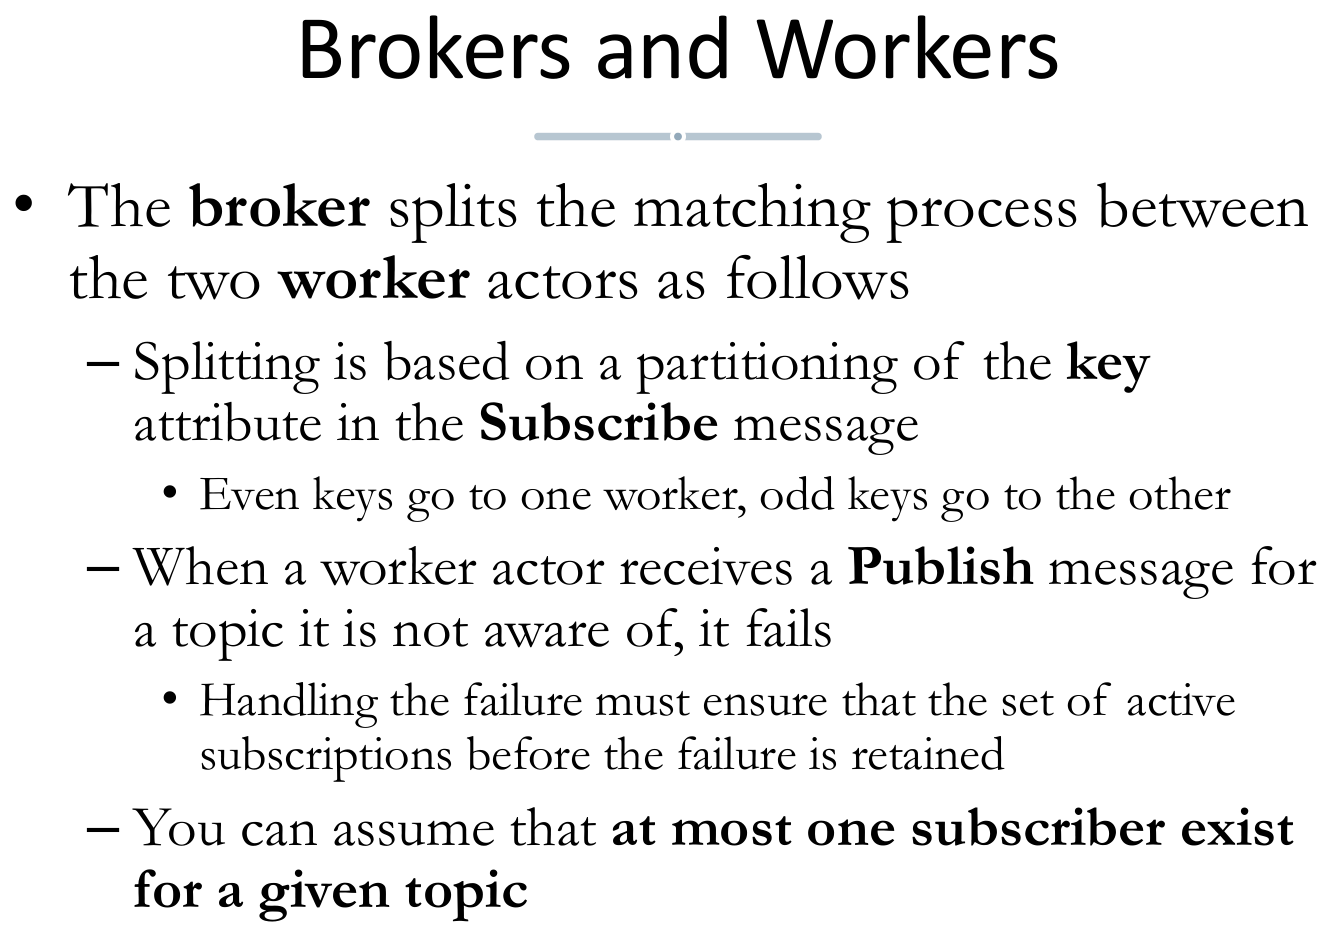
\includegraphics[width=0.75\textwidth]{img/chapter_01/eval22_pubsub_architecture.png}
\caption{Evaluation Lab 2022 Architecture: Broker partitioning subscriptions across even/odd workers, handling dynamic batching and supervisor recovery.}
\label{fig:eval22_architecture}
\end{figure}

\subsubsection{Complete Implementation}

\begin{lstlisting}[language=Java, caption={Message Definitions for Pub/Sub System}]
import akka.actor.ActorRef;
import java.io.Serializable;

public class Messages {
    public static class SubscribeMsg implements Serializable {
        private final String topic;
        private final int key;
        private final ActorRef subscriber;

        public SubscribeMsg(String topic, int key, ActorRef subscriber) {
            this.topic = topic;
            this.key = key;
            this.subscriber = subscriber;
        }
        public String getTopic() { return topic; }
        public int getKey() { return key; }
        public ActorRef getSubscriber() { return subscriber; }
    }

    public static class PublishMsg implements Serializable {
        private final String topic;
        private final int key;
        private final String payload;

        public PublishMsg(String topic, int key, String payload) {
            this.topic = topic;
            this.key = key;
            this.payload = payload;
        }
        public String getTopic() { return topic; }
        public int getKey() { return key; }
        public String getPayload() { return payload; }
    }

    public static class NotifyMsg implements Serializable {
        private final String payload;
        public NotifyMsg(String payload) { this.payload = payload; }
        public String getPayload() { return payload; }
    }

    public static class BatchMsg implements Serializable {
        private final boolean on;
        public BatchMsg(boolean on) { this.on = on; }
        public boolean isOn() { return on; }
    }
}
\end{lstlisting}

\begin{lstlisting}[language=Java, caption={WorkerActor with Fault Injection on Unknown Topics}]
import akka.actor.AbstractActor;
import akka.actor.Props;
import java.util.HashMap;
import java.util.Map;

public class WorkerActor extends AbstractActor {
    // Subscriptions map: Topic -> Subscriber ActorRef
    private final Map<String, ActorRef> subscriptions = new HashMap<>();

    public static Props props() {
        return Props.create(WorkerActor.class, WorkerActor::new);
    }

    @Override
    public Receive createReceive() {
        return receiveBuilder()
            .match(Messages.SubscribeMsg.class, msg -> {
                subscriptions.put(msg.getTopic(), msg.getSubscriber());
                System.out.println(self().path().name() + " registered topic: " + msg.getTopic());
            })
            .match(Messages.PublishMsg.class, msg -> {
                if (!subscriptions.containsKey(msg.getTopic())) {
                    System.err.println(self().path().name() + " fault: Unknown topic " + msg.getTopic());
                    throw new Exception("Unknown topic: " + msg.getTopic());
                }
                ActorRef sub = subscriptions.get(msg.getTopic());
                sub.tell(new Messages.NotifyMsg(msg.getPayload()), self());
            })
            .build();
    }
}
\end{lstlisting}

\begin{lstlisting}[language=Java, caption={BrokerActor with Dynamic Batching and Resume Supervision}]
import akka.actor.*;
import akka.japi.pf.DeciderBuilder;
import java.time.Duration;
import java.util.LinkedList;
import java.util.Queue;

public class BrokerActor extends AbstractActorWithStash {
    private final ActorRef workerEven;
    private final ActorRef workerOdd;
    private final Queue<Messages.PublishMsg> batchBuffer = new LinkedList<>();

    // Supervision Strategy: Resume on exception to retain subscriptions
    private static final SupervisorStrategy STRATEGY = new OneForOneStrategy(
        10,
        Duration.ofMinutes(1),
        DeciderBuilder
            .match(Exception.class, e -> SupervisorStrategy.resume())
            .build()
    );

    @Override
    public SupervisorStrategy supervisorStrategy() {
        return STRATEGY;
    }

    public BrokerActor() {
        this.workerEven = getContext().actorOf(WorkerActor.props(), "workerEven");
        this.workerOdd = getContext().actorOf(WorkerActor.props(), "workerOdd");
    }

    public static Props props() {
        return Props.create(BrokerActor.class, BrokerActor::new);
    }

    @Override
    public Receive createReceive() {
        return normalBehavior();
    }

    // Normal Behavior: immediate routing
    private Receive normalBehavior() {
        return receiveBuilder()
            .match(Messages.BatchMsg.class, msg -> {
                if (msg.isOn()) {
                    System.out.println("Broker transitioning to BATCH mode.");
                    getContext().become(batchBehavior());
                }
            })
            .match(Messages.SubscribeMsg.class, this::routeSubscription)
            .match(Messages.PublishMsg.class, this::routePublish)
            .build();
    }

    // Batch Behavior: buffer incoming publish events
    private Receive batchBehavior() {
        return receiveBuilder()
            .match(Messages.BatchMsg.class, msg -> {
                if (!msg.isOn()) {
                    System.out.println("Broker flushing batch (" + batchBuffer.size() + " messages).");
                    while (!batchBuffer.isEmpty()) {
                        routePublish(batchBuffer.poll());
                    }
                    getContext().become(normalBehavior());
                }
            })
            .match(Messages.SubscribeMsg.class, this::routeSubscription)
            .match(Messages.PublishMsg.class, batchBuffer::add)
            .build();
    }

    private void routeSubscription(Messages.SubscribeMsg msg) {
        if (msg.getKey() % 2 == 0) {
            workerEven.forward(msg, getContext());
        } else {
            workerOdd.forward(msg, getContext());
        }
    }

    private void routePublish(Messages.PublishMsg msg) {
        if (msg.getKey() % 2 == 0) {
            workerEven.forward(msg, getContext());
        } else {
            workerOdd.forward(msg, getContext());
        }
    }
}
\end{lstlisting}

---

\subsection{Evaluation Lab 2023 Solution: Sensor Data Processing with Policy Dispatching}

\subsubsection{Problem Specification}
Develop an industrial temperature monitoring pipeline in Akka with:
\begin{enumerate}
    \item \textbf{SensorDataProcessor Actors}: Maintain the running average of received temperature readings:
    \begin{equation}
    \bar{T}_{k} = \frac{(k-1)\bar{T}_{k-1} + T_k}{k}
    \end{equation}
    If a negative temperature reading is received, the processor raises an exception. Fault recovery must ensure the average temperature before failure is preserved, but the negative reading is excluded (\texttt{Resume}).
    \item \textbf{DispatcherActor}: Dynamically routes incoming readings according to two policies configurable via \texttt{DispatchLogicMsg}:
    \begin{itemize}
        \item \textbf{Load Balancing}: Permanently assigns each sensor to the least-loaded data processor.
        \item \textbf{Round Robin}: Rotates incoming readings sequentially across data processors.
    \end{itemize}
\end{enumerate}

\begin{figure}[htbp]
\centering
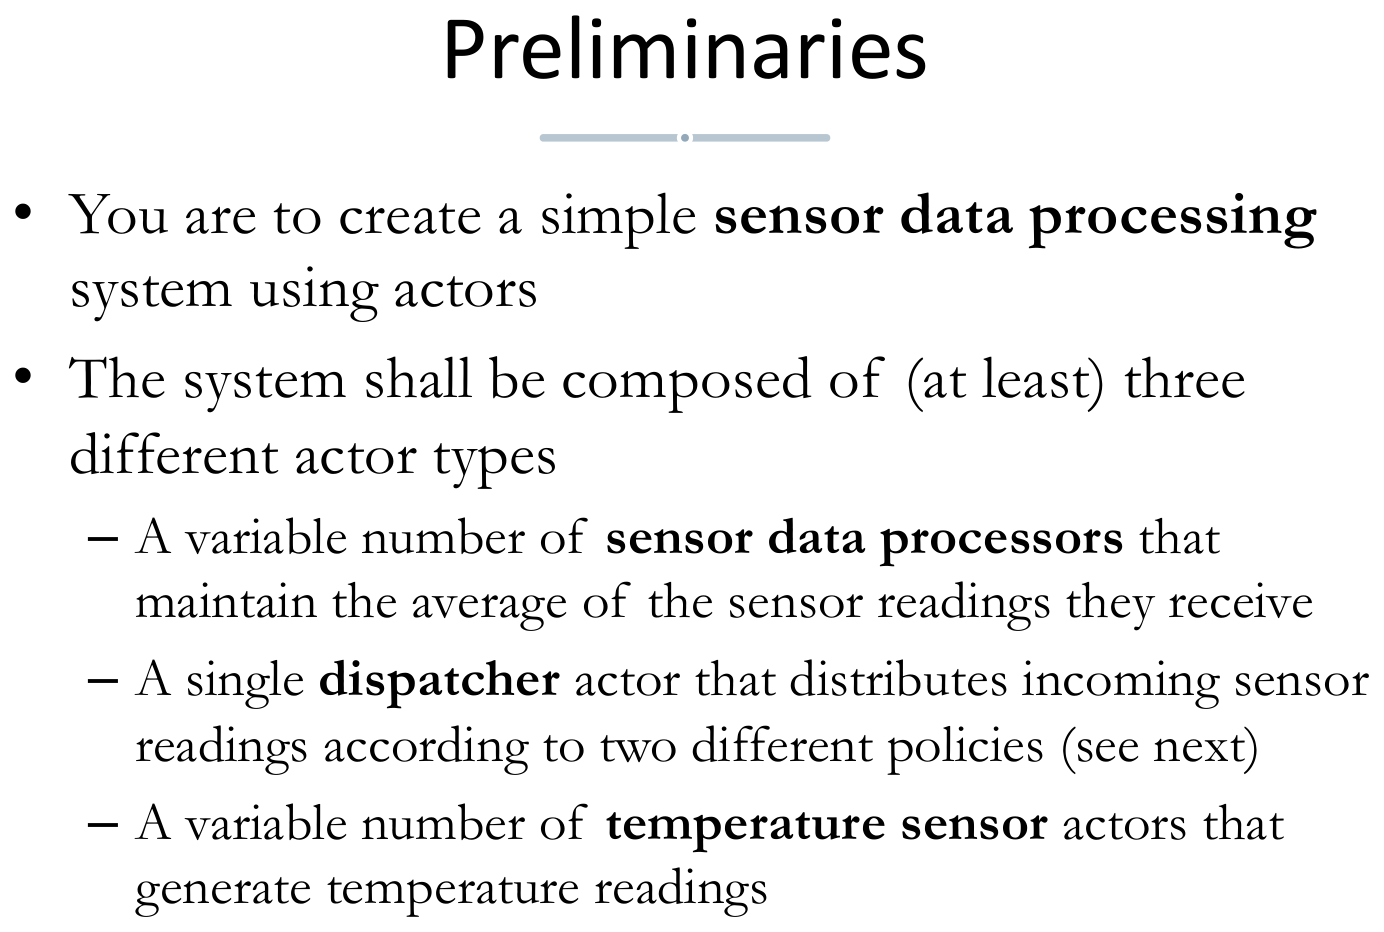
\includegraphics[width=0.75\textwidth]{img/chapter_01/eval23_sensor_architecture.png}
\caption{Evaluation Lab 2023 Architecture: Dispatcher routing sensor readings via dynamic Load Balancing or Round Robin to resilient Data Processors.}
\label{fig:eval23_architecture}
\end{figure}

\subsubsection{Complete Implementation}

\begin{lstlisting}[language=Java, caption={SensorProcessorActor with State Invariant Preservation}]
import akka.actor.AbstractActor;
import akka.actor.Props;

public class SensorProcessorActor extends AbstractActor {
    private double sum = 0.0;
    private int count = 0;

    public static Props props() {
        return Props.create(SensorProcessorActor.class, SensorProcessorActor::new);
    }

    @Override
    public Receive createReceive() {
        return receiveBuilder()
            .match(TemperatureMsg.class, msg -> {
                if (msg.getValue() < 0) {
                    System.err.println(self().path().name() + " rejecting invalid temperature: " + msg.getValue());
                    throw new IllegalArgumentException("Negative temperature invalid: " + msg.getValue());
                }
                count++;
                sum += msg.getValue();
                double currentAvg = sum / count;
                System.out.printf("%s -> Read: %.2f | New Running Avg: %.2f (Total readings: %d)%n",
                    self().path().name(), msg.getValue(), currentAvg, count);
            })
            .build();
    }
}
\end{lstlisting}

\begin{lstlisting}[language=Java, caption={DispatcherActor with Dynamic Routing Policies and Fault Recovery}]
import akka.actor.*;
import akka.japi.pf.DeciderBuilder;
import java.time.Duration;
import java.util.*;

public class DispatcherActor extends AbstractActor {
    private final List<ActorRef> processors;
    private final Map<ActorRef, ActorRef> sensorToProcessorMap = new HashMap<>();
    private final Map<ActorRef, Integer> processorLoadMap = new HashMap<>();
    private int roundRobinIndex = 0;
    private boolean isRoundRobin = true; // Default policy

    private static final SupervisorStrategy STRATEGY = new OneForOneStrategy(
        10,
        Duration.ofMinutes(1),
        DeciderBuilder
            .match(IllegalArgumentException.class, e -> SupervisorStrategy.resume())
            .build()
    );

    @Override
    public SupervisorStrategy supervisorStrategy() {
        return STRATEGY;
    }

    public DispatcherActor(int numProcessors) {
        this.processors = new ArrayList<>();
        for (int i = 0; i < numProcessors; i++) {
            ActorRef p = getContext().actorOf(SensorProcessorActor.props(), "processor-" + i);
            processors.add(p);
            processorLoadMap.put(p, 0);
        }
    }

    public static Props props(int numProcessors) {
        return Props.create(DispatcherActor.class, () -> new DispatcherActor(numProcessors));
    }

    @Override
    public Receive createReceive() {
        return receiveBuilder()
            .match(DispatchLogicMsg.class, msg -> {
                this.isRoundRobin = msg.isRoundRobin();
                System.out.println("Dispatcher switched logic to: " + 
                    (isRoundRobin ? "ROUND ROBIN" : "LOAD BALANCING"));
            })
            .match(TemperatureMsg.class, msg -> {
                ActorRef targetProcessor;
                if (isRoundRobin) {
                    targetProcessor = processors.get(roundRobinIndex);
                    roundRobinIndex = (roundRobinIndex + 1) % processors.size();
                } else {
                    ActorRef sensorSender = sender();
                    if (!sensorToProcessorMap.containsKey(sensorSender)) {
                        // Find processor with minimum assigned sensors
                        targetProcessor = processors.stream()
                            .min(Comparator.comparingInt(processorLoadMap::get))
                            .orElse(processors.get(0));
                        sensorToProcessorMap.put(sensorSender, targetProcessor);
                        processorLoadMap.put(targetProcessor, processorLoadMap.get(targetProcessor) + 1);
                    } else {
                        targetProcessor = sensorToProcessorMap.get(sensorSender);
                    }
                }
                targetProcessor.forward(msg, getContext());
            })
            .build();
    }
}
\end{lstlisting}



\end{document}
